%  template.tex for Biometrics papers
%
%  This file provides a template for Biometrics authors.  Use this
%  template as the starting point for creating your manuscript document.
%  See the file biomsample.tex for an example of a full-blown manuscript.

%  ALWAYS USE THE referee OPTION WITH PAPERS SUBMITTED TO BIOMETRICS!!!
%  You can see what your paper would look like typeset by removing
%  the referee option.  Because the typeset version will be in two
%  columns, however, some of your equations may be too long. DO NOT
%  use the \longequation option discussed in the user guide!!!  This option
%  is reserved ONLY for equations that are impossible to split across
%  multiple lines; e.g., a very wide matrix.  Instead, type your equations
%  so that they stay in one column and are split across several lines,
%  as are almost all equations in the journal.  Use a recent version of the
%  journal as a guide.
%
\documentclass[useAMS,usenatbib,referee]{biom}
%documentclass[useAMS]{biom}
%
%  If your system does not have the AMS fonts version 2.0 installed, then
%  remove the useAMS option.
%
%  useAMS allows you to obtain upright Greek characters.
%  e.g. \umu, \upi etc.  See the section on "Upright Greek characters" in
%  this guide for further information.
%
%  If you are using AMS 2.0 fonts, bold math letters/symbols are available
%  at a larger range of sizes for NFSS release 1 and 2 (using \boldmath or
%  preferably \bmath).
%
%  Other options are described in the user guide. Here are a few:
%
%  -  If you use Patrick Daly's natbib  to cross-reference your
%     bibliography entries, use the usenatbib option
%
%  -  If you use \includegraphics (graphicx package) for importing graphics
%     into your figures, use the usegraphicx option
%
%  If you wish to typeset the paper in Times font (if you do not have the
%  PostScript Type 1 Computer Modern fonts you will need to do this to get
%  smoother fonts in a PDF file) then uncomment the next line
%  \usepackage{Times}

%%%%% PLACE YOUR OWN MACROS HERE %%%%%

\def\bSig\mathbf{\Sigma}
\newcommand{\VS}{V\&S}
\newcommand{\tr}{\mbox{tr}}
\newcommand{\RNum}[1]{\uppercase\expandafter{\romannumeral #1\relax}}

%packages

\usepackage{amsmath}
%\usepackage{biblatex}
\usepackage{bm}
\usepackage{hyperref}
\usepackage{graphicx}
%\usepackage{natbib}

%  The rotating package allows you to have tables displayed in landscape
%  mode.  The rotating package is NOT included in this distribution, but
%  can be obtained from the CTAN archive.  USE OF LANDSCAPE TABLES IS
%  STRONGLY DISCOURAGED -- create landscape tables only as a last resort if
%  you see no other way to display the information.  If you do do this,
%  then you need the following command.

%\usepackage[figuresright]{rotating}

%%%%%%%%%%%%%%%%%%%%%%%%%%%%%%%%%%%%%%%%%%%%%%%%%%%%%%%%%%%%%%%%%%%%%

%  Here, place your title and author information.  Note that in
%  use of the \author command, you create your own footnotes.  Follow
%  the examples below in creating your author and affiliation information.
%  Also consult a recent issue of the journal for examples of formatting.

\title[Addressing Confounding and Measurement Error]{Addressing Confounding and Exposure Measurement Error Using Conditional Score Functions}

%  Here are examples of different configurations of author/affiliation
%  displays.  According to the Biometrics style, in some instances,
%  the convention is to have superscript *, **, etc footnotes to indicate
%  which of multiple email addresses belong to which author.  In this case,
%  use the \email{ } command to produce the emails in the display.

%  In other cases, such as a single author or two authors from
%  different institutions, there should be no footnoting.  Here, use
%  the \emailx{ } command instead.

%  The examples below correspond to almost every possible configuration
%  of authors and may be used as a guide.  For other configurations, consult
%  a recent issue of the the journal.

%  Single author -- USE \emailx{ } here so that no asterisk footnoting
%  for the email address will be produced.

%\author{John Author\emailx{email@address.edu} \\
%Department of Statistics, University of Warwick, Coventry CV4 7AL, U.K.}

%  Two authors from the same institution, with both emails -- use
%  \email{ } here to produce the asterisk footnoting for each email address

%\author{John Author$^{*}$\email{author@address.edu} and
%Kathy Authoress$^{**}$\email{email2@address.edu} \\
%Department of Statistics, University of Warwick, Coventry CV4 7AL, U.K.}

%  Exactly two authors from different institutions, with both emails
%  USE \emailx{ } here so that no asterisk footnoting for the email address
%  is produced.

%\author
%{John Author\emailx{author@address.edu} \\
%Department of Statistics, University of Warwick, Coventry CV4 7AL, U.K.
%\and
%Kathy Author\emailx{anotherauthor@address.edu} \\
%Department of Biostatistics, University of North Carolina at Chapel Hill,
%Chapel Hill, North Carolina, U.S.A.}

%  Three or more authors from same institution with all emails displayed
%  and footnoted using asterisks -- use \email{ }

%\author{John Author$^*$\email{author@address.edu},
%Jane Author$^{**}$\email{jane@address.edu}, and
%Dick Author$^{***}$\email{dick@address.edu} \\
%Department of Statistics, University of Warwick, Coventry CV4 7AL, U.K}

%  Three or more authors from same institution with one corresponding email
%  displayed

%\author{John Author$^*$\email{author@address.edu},
%Jane Author, and Dick Author \\
%Department of Statistics, University of Warwick, Coventry CV4 7AL, U.K}

%  Three or more authors, with at least two different institutions,
%  more than one email displayed

%\author{John Author$^{1,*}$\email{author@address.edu},
%Kathy Author$^{2,**}$\email{anotherauthor@address.edu}, and
%Wilma Flinstone$^{3,***}$\email{wilma@bedrock.edu} \\
%$^{1}$Department of Statistics, University of Warwick, Coventry CV4 7AL, U.K \\
%$^{2}$Department of Biostatistics, University of North Carolina at
%Chapel Hill, Chapel Hill, North Carolina, U.S.A. \\
%$^{3}$Department of Geology, University of Bedrock, Bedrock, Kansas, U.S.A.}

%  Three or more authors with at least two different institutions and only
%  one email displayed

\author{Bryan S. Blette$^{1}$, Peter B. Gilbert$^{2}$, and Michael G. Hudgens$^{1,*}$\email{mhudgens@email.unc.edu} \\ $^{1}$Department of Biostatistics, University of North Carolina at Chapel Hill
\\ Chapel Hill, NC, U.S.A. \\
$^{2}$Department of Biostatistics, University of Washington and Fred Hutchinson Cancer Research Center
\\ Seattle, Washington, U.S.A.}


\usepackage{Sweave}
\begin{document}
\Sconcordance{concordance:Biometrics-draft.tex:Biometrics-draft.rnw:%
1 152 1 1 0 361 1}


%  This will produce the submission and review information that appears
%  right after the reference section.  Of course, it will be unknown when
%  you submit your paper, so you can either leave this out or put in
%  sample dates (these will have no effect on the fate of your paper in the
%  review process!)

%\date{{\it Received October} 2007. {\it Revised February} 2008.  {\it
%Accepted March} 2008.}

%  These options will count the number of pages and provide volume
%  and date information in the upper left hand corner of the top of the
%  first page as in published papers.  The \pagerange command will only
%  work if you place the command \label{firstpage} near the beginning
%  of the document and \label{lastpage} at the end of the document, as we
%  have done in this template.

%  Again, putting a volume number and date is for your own amusement and
%  has no bearing on what actually happens to your paper!

%\pagerange{\pageref{firstpage}--\pageref{lastpage}}
%\volume{64}
%\pubyear{2008}
%\artmonth{December}

%  The \doi command is where the DOI for your paper would be placed should it
%  be published.  Again, if you make one up and stick it here, it means
%  nothing!

%\doi{10.1111/j.1541-0420.2005.00454.x}

%  This label and the label ``lastpage'' are used by the \pagerange
%  command above to give the page range for the article.  You may have
%  to process the document twice to get this to match up with what you
%  expect.  When using the referee option, this will not count the pages
%  with tables and figures.

\label{firstpage}

%  put the summary for your paper here

\begin{abstract}
Confounding and measurement error are common barriers to drawing causal inference. While there are broad methodologies for addressing each phenomenon individually, confounding and measurement biases frequently co-occur and there is a paucity of methods that address them simultaneously. The few existing methods that do so rely on supplemental data or strong distributional and extrapolation assumptions to correct for measurement error. In this paper, methods are derived which instead leverage the likelihood structure under classical additive measurement error to draw inference using only measured variables. Three estimators are proposed based on g-computation, inverse probability weighting, and doubly-robust estimation techniques. The estimators are shown to be consistent and asymptotically normal and the doubly-robust estimator is shown to exhibit its namesake property. The methods perform well in finite samples under both confounding and measurement error as demonstrated by simulation studies. The proposed doubly-robust estimator is applied to study the effects of two biomarkers on HIV-1 infection using data from the HVTN 505 vaccine trial.
\end{abstract}

%  Please place your key words in alphabetical order, separated
%  by semicolons, with the first letter of the first word capitalized,
%  and a period at the end of the list.
%

\begin{keywords}
Causal inference; Confounding; G-formula; HIV/AIDS;
Marginal structural models; Measurement error.
\end{keywords}

%  As usual, the \maketitle command creates the title and author/affiliations
%  display

\maketitle

%  If you are using the referee option, a new page, numbered page 1, will
%  start after the summary and keywords.  The page numbers thus count the
%  number of pages of your manuscript in the preferred submission style.
%  Remember, ``Normally, regular papers exceeding 25 pages and Reader Reaction
%  papers exceeding 12 pages in (the preferred style) will be returned to
%  the authors without review. The page limit includes acknowledgements,
%  references, and appendices, but not tables and figures. The page count does
%  not include the title page and abstract. A maximum of six (6) tables or
%  figures combined is often required.''

%  You may now place the substance of your manuscript here.  Please use
%  the \section, \subsection, etc commands as described in the user guide.
%  Please use \label and \ref commands to cross-reference sections, equations,
%  tables, figures, etc.
%
%  Please DO NOT attempt to reformat the style of equation numbering!
%  For that matter, please do not attempt to redefine anything!

\section{Introduction}
\label{s:intro}

Confounding bias and measurement error are common barriers to identification, estimation, and inference of causal effects. These phenomena often occur together, but are rarely both addressed in an analysis, with researchers typically focusing on whichever is more egregious in their study or ignoring both entirely. The last few decades witnessed a proliferation of interest in and development of methods for causal inference and a parallel trend for methods accounting for measurement error, but comparatively few methods exist at the important intersection of these fields.

The measurement error literature is commonly split into (i) functional methods, which make no or limited assumptions on the distribution of mismeasured variables, and (ii) structural methods, which make explicit distributional assumptions~\citep{carroll2006}. Several causal methods based on structural approaches have been developed (\citealp{kuroki2014,edwards2015multiple,braun2017}; \citealp*{hong2017}). Likewise, three of the four most popular functional methods (regression calibration, SIMEX, and methods based on instrumental variables) have been adapted to a variety of causal problems (\citealp*{vansteelandt2009}; \citealp{cole2010,kendall2015,lockwood2015,kyle2016,wu2019}). These methods all rely on either supplemental data, such as replication, validation, or instrumental data, or on strong distributional and extrapolation assumptions to draw inference.

In contrast, the fourth main functional approach, that of score functions, leverages the likelihood structure under classical additive measurement error to draw inference without supplemental data or such strong assumptions. Despite this advantage, this method has only been adapted to perform causal inference in very limited capacity, perhaps due to its increased complexity over other functional approaches and lack of available software. In particular, \citet*{mccaffrey2013} suggested using weighted conditional score equations to correct for measurement error in confounders and the approach was eventually implemented in \citet{shu2019}. In this paper, we expand this methodology in multiple directions, considering exposure/treatment measurement error and defining g-formula, IPW, and doubly-robust estimators.

The proposed methods are motivated by the HVTN 505 vaccine trial. This trial evaluated a candidate HIV vaccine and stopped administering immunizations in 2013 after reaching predetermined cutoffs for futility~\citep{hammer2013}. However, follow-up analyses of trial data described several correlates of risk among trial participants~\citep{decamp2017,janes2017,fong2018,neidich2019}. Some of these biomarkers correspond to possible target immune responses for future vaccine trials, but their causal effects on HIV-1 infection have not been described. The methods derived in this paper are motivated by this problem, where the biomarkers are measured with error and their effects are likely subject to confounding, but there is no supplemental data available.

This paper proceeds as follows. In Section 2, notation and the estimand are defined. In Section 3, assumptions are stated and three estimators that adjust for concurrent confounding and exposure measurement error using a conditional score approach are proposed. In Section 4, the proposed estimators are evaluated in a simulation study and in Section 5, one of the estimators is applied to study two biomarkers collected in the HVTN 505 vaccine trial. Section 6 concludes with a discussion of the advantages and limitations of the proposed methods.

\section{Notation and Estimand}
\label{s:notation}

Suppose there are $m$ exposures/treatments of interest which may or may not be measured correctly. Let $\bm{A}_{i} = (A_{i1}, A_{i2}, ..., A_{im})$ be a row vector denoting the true exposures for individual $i$ and $\bm{A}^{*}_{i} =  (A^{*}_{i1}, A^{*}_{i2}, ..., A^{*}_{im})$ be the corresponding set of measured exposures. Suppose only the first $j$ exposures are measured with error, such that $A_{ik} = A^{*}_{ik}$ for $k > j$ for all individuals. For example, in the HVTN 505 trial, a biomarker of interest $A$ is antibody-dependent cellular phagocytosis activity. This biomarker was not observed exactly, but an imperfect phagocytic score $A^{*}$ was measured using flow cytometry analysis. Exposures subject to measurement error are assumed to be continuous random variables, while exposures known to be correctly measured may be continuous or discrete. Let $Y_{i}$ be the outcome of interest. Define $Y_{i}(\bm{a})$ to be the potential outcome under treatments $\bm{A} = \bm{a} = (a_{1}, a_{2}, ..., a_{m})$. Since there is at least one continuous exposure, each individual has infinite potential outcomes. Let $\bm{L}_{i} =  (L_{i1}, L_{i2}, ..., L_{ip})$ represent a vector of baseline covariates measured prior to the exposures. Assume that $n$ i.i.d. copies of the random variables $(\bm{L}, \bm{A}^{*}, Y)$ are observed.

Consider the marginal structural model (MSM)
\begin{equation}
    g(\text{E}[Y(\bm{a})]) = \gamma (1, \bm{a})^{T}
\end{equation}
where $g$ is a link function for an exponential family density, e.g., $g(\cdot) = \text{logit}(\cdot)$. The MSM parameter $\gamma = (\gamma_{0}, ..., \gamma_{m})$ is a row vector of length $m+1$ which quantifies the effects of the exposures on the outcome. The parameter $\gamma_{0}$ describes the mean outcome when all exposures are set to 0, which may or may not be of interest depending on the exposures being studied. The linear structure of the MSM is key to matching the conditional score framework described in the next section; more complicated specifications are considered in Web Appendix D.

\begin{figure}
\centering
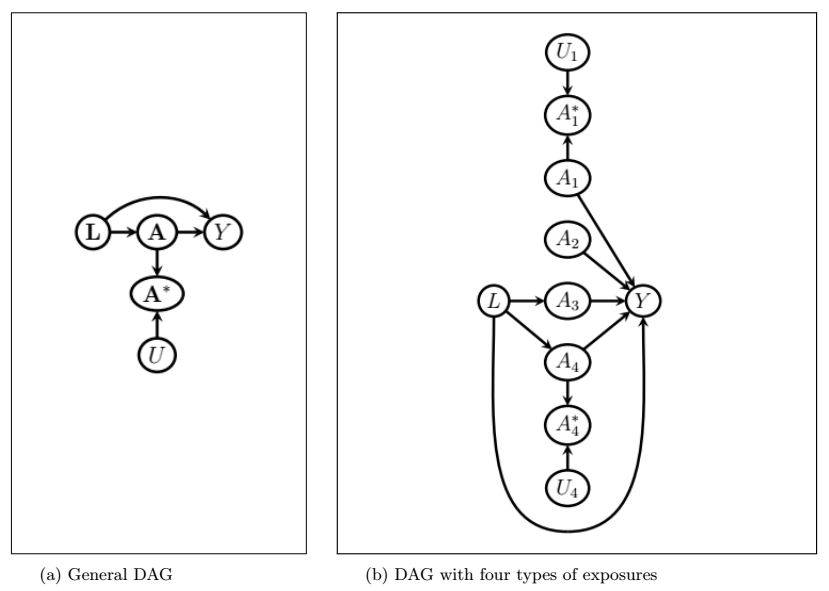
\includegraphics[width=6in]{Paper1_Fig1.png}
\caption{Directed Acyclic Graphs (DAGs) corresponding to the problem setup, with variables defined in section 2 and $U$ corresponding to measurement error. (a) A general DAG where $\bm{A}$ is a vector of exposures, some of which may be mismeasured (indicated by the arrow to $\bm{A}^{*}$) and some of which may be subject to confounding bias (indicated by the arrow from $\bm{L}$). (b) A DAG for a specific exposure vector with four different types of exposures: mismeasured and unconfounded ($A_{1}$), correctly measured and unconfounded ($A_{2}$), correctly measured and confounded ($A_{3}$), and mismeasured and confounded ($A_{4}$). Each of these four types of exposures can be handled by the proposed modeling framework.}
\label{fig:one}
\end{figure}

A compressed version of the directed acyclic graph (DAG) for this setup is presented in Figure~\ref{fig:one}(a). Note that the DAG implies non-differential measurement error with respect to the outcome, i.e., the exposure error and the outcome are independent because $\bm{A}^{*}$ is a collider on all paths connecting them. In Figure~\ref{fig:one}(b), the DAG is expanded to show the four types of exposures which may belong to $\bm{A}$: unconfounded and correctly measured, unconfounded and mismeasured, confounded and correctly measured, and confounded and mismeasured. Many existing methods focus on only mismeasured exposures or on a set of correctly measured exposures with one additional mismeasured exposure; the methods developed in this paper provide a more broadly usable modeling framework where all four types of exposures can be studied simultaneously.

\section{Methods}
\label{s:methods}

\subsection{Review of Conditional Score Approach}

The proposed methods combine existing methods for (i) correcting exposure measurement error using conditional score equations (CSME) and (ii) adjusting for confounding using g-formula, inverse probability weighting (IPW), and doubly-robust techniques. To begin, CSME methodology is briefly reviewed.

Assume that the outcome conditional on exposures and covariates can be represented as an exponential-family density~\citep{mccullagh2018}, i.e., $f(y | \bm{a}, \bm{l}, \Theta) = \exp [ \{y\eta - \mathcal{D}(\eta)\}/ \phi + c(y, \phi) ]$ where $\eta = \beta_{0} + \bm{a}\beta_{a} + \bm{l}\beta_{l}$, $\mathcal{D}$ and $c$ are functions, $\bm{a}$ and $\bm{l}$ are realizations of the random variables $\bm{A}$ and $\bm{L}$, and $\Theta = (\beta_{0}, \beta^{T}_{a}, \beta^{T}_{l}, \phi)$ represents the parameters to be estimated. Assume a classical additive measurement error model $\bm{A}^{*} = \bm{A} + \epsilon_{me}$, where $\epsilon_{me}$ is multivariate normal with mean zero and covariance matrix $\Sigma_{me}$. To account for $A_{j+1}, ...,  A_{m}$ being correctly measured, assume $\Sigma_{me}$ has the block diagonal form
\begin{equation*}
    \Sigma_{me} =
    \begin{bmatrix}
    \Sigma_{e} & 0_{j,m-j} \\
    0_{m-j,j} & 0_{m-j,m-j}
    \end{bmatrix}
\end{equation*}
where $\Sigma_{e}$ is the measurement error covariance matrix for exposures $A_{1},...,A_{j}$ and $0_{a,b}$ denotes an $a \times b$ matrix of zeros.

The CSME approach leverages the fact that $\bm{\Delta}_{i} = \bm{A}^{*}_{i} + Y_{i}(\Sigma_{me}\beta_{a})^{T}/\phi$ is a sufficient statistic for $\bm{A}_{i}$. This implies that the score equations from the likelihood conditional on $\bm{\Delta}_{i}$ yield consistent estimators for $\beta_{a}$ that only depend on the observed data. The form of the score equations depends on the model specification; the general form is given by
\begin{equation}
    \psi(Y_{i}, \bm{L}_{i}, \bm{A}^{*}_{i}, \Theta) =
    \begin{bmatrix}
       \{ Y_{i} - \text{E}(Y_{i} | \bm{L}_{i}, \bm{\Delta}_{i}) \} (1, \bm{L}_{i}, \bm{\Delta}_{i})^{T} \\
        \phi - \{ Y_{i} - \text{E}(Y_{i} | \bm{L}_{i}, \bm{\Delta}_{i}) \}^{2} / \{ \text{Var}(Y_{i} | \bm{L}_{i}, \bm{\Delta}_{i}) / \phi \}
    \end{bmatrix}
\end{equation}
where $\text{E}(Y_{i} | \bm{L}_{i}, \bm{\Delta}_{i}) = \partial \mathcal{D}_{*} / \partial \eta_{*}$, $\text{Var}(Y_{i} | \bm{L}_{i}, \bm{\Delta}_{i}) = \phi \partial^{2} \mathcal{D}_{*} / \partial \eta^{2}_{*}$. The density of the outcome conditional on covariates and the sufficient statistic is also an exponential-family density with parameters $\eta_{*} = \beta_{0} + \bm{\delta}\beta_{a} + \bm{l}\beta_{l}$, $\mathcal{D}_{*}(\eta_{*}, \phi, \beta_{a}^{T}\Sigma_{me}\beta_{a}) = \phi \log \bigg[ \int \exp \{ y\eta_{*}/\phi + c_{*}(y, \phi,  \beta_{a}^{T}\Sigma_{me}\beta_{a}) \} d\mu y \bigg]$, and $c_{*}(y, \phi, \beta_{a}^{T}\Sigma_{me}\beta_{a}) = c(y, \phi) - \frac{1}{2}(y/\phi)^{2}\beta_{a}^{T}\Sigma_{me}\beta_{a}$, where $\bm{\delta}$ is a realization of $\bm{\Delta}$. This procedure can be extended to handle interaction terms~\citep{dagalp2001} resulting in estimating equations of the form
\begin{equation*}
    \psi(Y_{i}, \bm{L}_{i}, \bm{A}^{*}_{i}, \Theta) =
    \begin{bmatrix}
       \{ Y_{i} - \text{E}(Y_{i} | \bm{L}_{i}, \bm{\Delta}_{i}) \} (1, \bm{L}_{i}, \bm{\Delta}_{i}, \bm{L}_{i} \otimes \bm{\Delta}_{i})^{T} \\
        \phi - \{ Y_{i} - \text{E}(Y_{i} | \bm{L}_{i}, \bm{\Delta}_{i}) \}^{2} / \{ \text{Var}(Y_{i} | \bm{L}_{i}, \bm{\Delta}_{i}) / \phi \}
    \end{bmatrix}
\end{equation*}
where now $\eta = \beta_{0} + \bm{a}\beta_{a} + \bm{l}\beta_{l} + \bm{a}\beta_{al}\bm{l}^{T}$, $\beta_{al}$ is an $m \times p$ matrix of interaction parameters, $\bm{\Delta}_{i} = \bm{A}_{i}^{*} + Y_{i}\{ \Sigma_{me}(\beta_{a} + \beta_{al}\bm{L}_{i}^{T}) \}^{T}/\phi$, and appropriate elements of $\beta_{al}$ can be constrained to zero such that only relevant interactions are included in the model. Here $\Theta = (\beta_{0}, \beta^{T}_{a}, \beta^{T}_{l}, \text{vec}(\beta_{al}), \phi)$, where $\text{vec}$ maps the nonzero elements of the interaction parameter matrix reading left to right then top to bottom to a row vector. Define $\bm{L}_{i} \otimes \Delta_{i}$ as a vector of length $\dim(\text{vec}(\beta_{al}))$ containing the product of the kth element of $L_{i}$ and the rth element of $\bm{\Delta}_{i}$ if and only if the (r, k) element of $\beta_{al}$ is not constrained to be zero.

Next, three methods will be proposed which combine the CSME approach with common causal inference techniques in order to adjust for confounding and measurement error simultaneously. The proposed methods rely on the CSME modeling assumptions stated above as well as a standard set of assumptions used in causal inference: (i) causal consistency, $Y = Y(\bm{a})$ when $\bm{A} = \bm{a}$; (ii) conditional exchangeability, $Y(\bm{a}) \perp \!\!\! \perp \bm{A} | \bm{L}$; and (iii) positivity, $f(\bm{a} | \bm{l}) > 0$ for all $\bm{l}$ such that $dF_{\bm{L}}(\bm{l}) > 0$, where $F_{\bm{L}}$ is the cumulative distribution function of $\bm{L}$. As represented in the DAG in Figure~\ref{fig:one}(a), the exposure measurement error is assumed non-differential with respect to the outcome. Finally, assume that the outcome and covariates are not measured with error and that there is no model mis-specification throughout unless otherwise stated.

\subsection{G-formula CSME Estimator}

\sloppy The first proposed method combines the g-formula with the CSME method. Let $\bm{A}_{(-j)} = (A_{1}, ..., A_{j-1}, A_{j+1}, ..., A_{m})$ be the vector of treatments excluding $A_{j}$ and let $Y(a_{j}, \bm{a}_{(-j)})$ be the potential outcome under $A_{j} = a_{j}$ and $\bm{A}_{(-j)} = \bm{a}_{(-j)}$. Then the g-formula CSME estimator of $\gamma_{j}$ for $j = 1,...,m$ is
\begin{align*}
    \hat{\gamma_{j}} &= \hat{\text{E}}\{ Y(a_{j}, \bm{a}_{(-j)}) \} - \hat{\text{E}}\{ Y(a_{j} - 1, \bm{a}_{(-j)}) \} \\
    &= \int_{\bm{l} \in \bm{L}} \hat{\text{E}}(Y | A_{j} = a_{j}, \bm{A}_{(-j)} = \bm{a}_{(-j)}, \bm{L}) d\hat{F}_{\bm{L}}(\bm{l}) \\
    &- \int_{\bm{l} \in \bm{L}} \hat{\text{E}}(Y | A_{j} = a_{j} - 1, \bm{A}_{(-j)} = \bm{a}_{(-j)}, \bm{L}) d\hat{F}_{\bm{L}}(\bm{l})
\end{align*}
where the outcome predictions are from a fit CSME model with relevant interaction terms and $a_{j}$ and $\bm{a}_{(-j)}$ are constants. Equivalently, this estimator is a solution to the estimating equation $\sum_{i=1}^{n} \psi_{GF-CSME}(Y_{i}, \bm{L}_{i}, \bm{A}_{i}^{*}, \Sigma_{me}, \Theta) = 0$, where $\Theta = (\beta_{0}, \beta^{T}_{a}, \beta^{T}_{l}, vec(\beta_{al}), \phi, \gamma_{1}, ..., \gamma_{m})$ and

\begin{equation}
    \psi_{GF-CSME}(Y_{i}, \bm{L}_{i}, \bm{A}^{*}_{i}, \Sigma_{me}, \Theta) =
    \begin{bmatrix}
       \{ Y_{i} - \text{E}(Y_{i} | \bm{L}_{i}, \bm{\Delta}_{i}) \} (1, \bm{L}_{i}, \bm{\Delta}_{i}, \bm{L}_{i} \otimes \bm{\Delta}_{i})^{T} \\
        \phi - \{ Y_{i} - \text{E}(Y_{i} | \bm{L}_{i}, \bm{\Delta}_{i}) \}^{2} / \{ \text{Var}(Y_{i} | \bm{L}_{i}, \bm{\Delta}_{i}) / \phi \} \\
        \beta_{a_{1}\bm{l}}\bm{l}_{i}^{T} + \beta_{a_{1}} - \gamma_{1} \\
        \vdots \\
        \beta_{a_{m}\bm{l}}\bm{l}_{i}^{T} + \beta_{a_{m}} - \gamma_{m} \\
    \end{bmatrix}
\end{equation}
where notation for the coefficients from the CSME method are expanded as $\beta_{a} = (\beta_{a_{1}},...,\beta_{a_{m}})^{T}$ and $\beta_{al} = (\beta_{a_{1}l}, ..., \beta_{a_{m}l})^{T}$, where $\beta_{a_{j}l}$ is the $1 \times p$ vector of parameters corresponding to interactions between $a_{j}$ and covariates in $\textbf{L}$ for $j = 1,...,m$ (with zeroes for interactions not included in the outcome model).

\subsection{IPW CSME Estimator}

Since the CSME approach is defined using estimating equations, it's relatively straightforward to define an IPW extension. In particular, consider an estimator of the parameters of interest that solves $\sum_{i=1}^{n} \psi_{IPW-CSME}(Y_{i}, \bm{L}_{i}, \bm{A}^{*}_{i}, \Sigma_{me}, \Theta) = 0$ where:

\begin{equation}
    \psi_{IPW-CSME}(Y_{i}, \bm{L}_{i}, \bm{A}^{*}_{i}, \Sigma_{me}, \Theta) =
    \begin{bmatrix}
       SW_{i} \{ Y_{i} - E(Y_{i} | \bm{\Delta}_{i}) \} (1, \bm{\Delta}_{i})^{T} \\
       SW_{i} \left [ \phi - \{ Y_{i} - E(Y_{i} | \bm{\Delta}_{i})\}^{2} / \{ Var(Y_{i} | \bm{\Delta}_{i}) / \phi \} \right ]
    \end{bmatrix}
\end{equation}
\begin{equation*}
SW_{i} = \frac{f(A_{i1}, A_{i2}, ..., A_{in})}{f(A_{i1}, A_{i2}, ..., A_{in}) | \bm{L}_{i})} = \frac{f(A_{i1})f(A_{i2} | A_{i1}), ..., f(A_{in} | A_{i1}, ..., A_{i,n-1})}{f(A_{i,1} | \bm{L}_{i})f(A_{i2} | A_{i1}, \bm{L}_{i}), ..., f(A_{in} | A_{i1}, ..., A_{i,n-1}, \bm{L}_{i})}
\end{equation*}
and the $\beta_{0}$ and $\beta_{a}$ parameters nested within the conditional expectation and variance can be changed to $\gamma_{0}$ and $\gamma_{(-0)}$ such that $\hat{\gamma}$ is the solution to (4).

Rather than the Markov factorization given above, most MSM with multiple treatments use weights of the form $SW_{i} = \prod_{j=1}^{m} f(A_{ij}) / f(A_{ij} | \bm{L}_{i})$ as originally described by \citet{hernan2001}, which assumes that the treatments are independent conditional on $\bm{L}$. For the simulations and application of this paper, this assumption will be made, but note that such a simplification may be dubious in various applications and will not hold if there are direct arrows between treatments in the DAG. For examples of estimating the joint propensity of various dependent exposures using mixed models, see \citet{tchetgen2012}, \citet{perez2014}, or \citet*{liu2016}. In the remainder of this paper, weights for continuous treatments will be estimated using a ratio of normal densities, but other methods~\citep{hirano2004} and more flexible choices for weight models~\citep{naimi2014} can also be used in general.

Note that since the weighting eliminates confounding, the estimating equations of (4) are actually simpler than (2), since covariates $\bm{L}$ do not need to be included in the outcome model. The new forms of the conditional expectation and variance follow from setting $\eta_{*} = \beta_{0} + \bm{\delta}\beta_{a}$ in the equations in Section 3.1. Solving (4) yields estimates of the parameters of the MSM (1) with an additional dispersion parameter estimate.

Estimating the weights provides an additional challenge in that the exposure measurement error has another opportunity to introduce bias. Fortunately, the exposures are now the propensity model(s) outcomes, and measurement error is usually much less serious for a model outcome than for model covariates~\citep{carroll2006}. In Web Appendix A, the proposed IPW CSME estimator is shown to be consistent even when the propensity models are fit using the mismeasured exposures without correction, under certain assumptions.

\subsection{Doubly-Robust CSME Estimator}

In the absence of measurement error, both the g-formula and IPW methods rely on model specifications that may not be correct in practice. The g-formula provides consistent estimation of potential outcome means only when the outcome model with exposures and confounders is correctly specified. Likewise, the IPW estimator is consistent only when the propensity score model is correctly specified. In contrast, doubly-robust (DR) estimators entail specifying both propensity and outcome models, but remain consistent if one is misspecified and the other is not (\citealp*{robins1994}; \citealp{lunceford2004,bang2005}).

A DR estimator for the additive measurement error setting can be written similarly to those described in \citet{robins2000b} and \citet{neugebauer2005} as the solution to the set of estimating equations $\sum_{i=1}^{n} \psi_{DR-CSME}(Y_{i}, \bm{L}_{i}, \bm{A}^{*}_{i}, \Theta) = 0$ where:

\begin{equation*}
    \psi_{DR-CSME}(Y_{i}, \bm{L}_{i}, \bm{A}^{*}_{i}, \Theta) =
    \begin{bmatrix}
       SW_{i} \{ Y_{i} - E(Y_{i} | \bm{\Delta}_{i}) - Q(\bm{A}_{i}, \bm{L}_{i}) \} + \int_{\bm{a}} h(\bm{a})Q(\bm{a}, \bm{L}_{i})d\mu (\bm{a}) \\
       SW_{i} \{ Y_{i} - E(Y_{i} | \bm{\Delta}_{i}) - Q(\bm{A}_{i}, \bm{L}_{i}) \} \bm{\Delta}_{i} + \int_{\bm{a}} h(\bm{a})Q(\bm{a}, \bm{L}_{i})d\mu (\bm{a})
    \end{bmatrix},
\end{equation*}
$h(\bm{a})$ is the numerator of the stabilized weights, $d\mu (\bm{a})$ is a Lebesgue measure, and $Q(\bm{A}, \bm{L})$ is a function of $\bm{A}$ and $\bm{L}$. This estimator is doubly-robust in the sense that it is consistent if either the weights $SW$ are derived from correctly specified propensity models or if the outcome regression is a correctly specified CSME model, given by $Q(\bm{A}, \bm{L}) = \beta_{0} + \beta_{a}\bm{A} + \beta_{l}\bm{L} + \beta_{al}(\bm{A} \otimes \bm{L}^{T}) - \psi^{T}(1, \bm{A}^{T})^{T}$.

\subsection{Handling Unknown Measurement Error Variance}

Although the proposed methods require no supplemental data and no distributional assumption on the true exposures $\bm{A}$, they do require a priori knowledge of the measurement error covariance matrix. Sometimes, this will be known from properties of the measurement tools (e.g., some bioassays, certain widely studied survey instruments) or will be available from a prior study. Here, some guidelines are provided for analyses where this matrix is unknown.

Firstly, there are many types of studies for which the covariance matrix should be diagonal (i.e., the measurement errors should be uncorrelated). For example, biological assays taken on different samples and analyzed by separate machines/researchers should have uncorrelated measurement errors, and different assays taken on the same sample may often have uncorrelated or very weakly correlated measurement errors. For other types of data such as survey responses, analysts should be more cautious, noting that response bias, recall bias, and other forms of measurement error in survey instruments may be correlated within individuals.

Many studies do have a small amount of supplemental data, namely replicates of the potentially mismeasured variables. These replicates can be used to estimate $\Sigma_{me}$ as described in \citet{carroll2006}. Suppose there are $k_{i}$ replicates of the mismeasured exposures, $\bm{A}^{*}_{i1}, ..., \bm{A}^{*}_{ik_{i}}$ with mean for individual $i$ notated as $\bm{A}^{*}_{i.}$. Then an estimator for the measurement error covariance is given by:
\begin{equation*}
    \hat{\Sigma}_{me} = \frac{\sum_{i=1}^{n} \sum_{j=1}^{k_{i}} (\bm{A}^{*}_{i} - \bm{A}^{*}_{i.})(\bm{A}^{*}_{i} - \bm{A}^{*}_{i.})^{T}}{\sum_{i=1}^{n}(k_{i} - 1)}
\end{equation*}
noting that when replicates are available, some of the existing methods described in the introduction are applicable and should give similar results to the proposed methods.

When no replicates are available and there is no prior knowledge of $\Sigma_{me}$, the proposed methods can still be used in the context of a sensitivity analysis. Often an upper bound for measurement error variance of individual variables can be ascertained - it is atypical for measurement error variance to be higher than the variance of a variable itself, for example. Once upper bounds are identified or chosen, repeating the proposed methods under a few reasonable $\Sigma_{me}$ specifications yields a sensitivity analysis showing how robust the effect sizes and confidence intervals are to increasing additive measurement error; this procedure is more straightforward when the matrix is small and diagonal and becomes difficult to interpret as the number of parameters grows.

\subsection{Large-Sample Properties and Variance Estimation}

In Web Appendix A, each of the three proposed estimators are shown to be consistent and asymptotically normal by showing they are M-estimators and that their corresponding estimating functions have expectation 0~\citep{stefanski2002}. In addition, the DR estimator is shown to be consistent when only one of the propensity and outcome models is correctly specified. Finally, the proposed estimators are shown to be generalizations of existing popular estimators used in the no measurement error setting.

Since each proposed estimator is an M-estimator, consistent estimators of their asymptotic variances are given by the empirical sandwich variance technique. Estimating equations corresponding to the estimation of weights (and $\hat{\Sigma}_{me}$ if estimated) should be added to the estimating equation stacks for each method to achieve nominal coverage rates. The geex R package~\citep{saul2017} streamlines variance estimation for M-estimators and is used in the simulation and application sections. Wald $100(1-\alpha)\%$ confidence intervals for the parameters of interest are then given by $\hat{\psi}_{i} \pm z_{1-\alpha/2} SE(\hat{\psi}_{i})$ where $z_q$ is the q-quantile of the standard normal distribution. Wald hypothesis testing procedures can be defined similarly.

\section{Simulation Study}

The performance of the proposed methods was evaluated in two simulation studies. The first simulation compared the proposed g-formula CSME and IPW CSME approaches to standard methods within a scenario where confounding and additive exposure measurement error were present. A total of 2000 data sets of $n = 800$ individuals were simulated, each with the following variables and distributions: a confounder $L_{1} \sim \text{Binom}(0.5)$, a second confounder $L_{2} \sim \text{Binom}(0.35)$, first true exposure $A_{1} \sim \mathcal{N}(4 + L_{1}, 1)$, second true exposure $A_{2} \sim \mathcal{N}(1.25 + 0.5L_{2}, 0.5)$, third true exposure $A_{3} \sim \mathcal{N}(2.5, 0.7)$ and an outcome $Y \sim \mathcal{N}(-0.1 + 0.3A_{1} + 0.2L_{1} - 0.4A_{2} - 0.3L_{2} - 0.05A_{3} - 0.15A_{1}L_{1} - 0.2A_{2}L_{2}, 0.5)$ such that $E[Y(a_{1}, a_{2}, a_{3})] = \psi_{0} + \psi_{1}a_{1} + \psi_{2}a_{2} + \psi_{3}a_{3} = -0.1 + 0.225a_{1} - 0.47a_{2} - 0.05a_{3}$. The second exposure $A_{2}$ was allowed to be correctly measured, while $A_{1}$ and $A_{3}$ were subject to additive measurement error simulated as $A_{1}^{*} \sim \mathcal{N}(A_{1}, 0.3)$ and $A_{3}^{*} \sim \mathcal{N}(A_{3}, 0.5)$ (such that the measurement error covariance matrix was diagonal).

Six methods were compared in performance estimating $\psi_{1}$, $\psi_{2}$, and $\psi_{3}$ using the observed data $\{ Y, A_{1}^{*}, A_{2}, A^{*}_{3}, L_{1}, L_{2} \}$. These methods were: (i) linear regression specifying Y as a function of $A_{1}^{*}, A_{2}, A^{*}_{3}, L_{1}, L_{2}$ and the interactions between $A_{1}^{*}$ and $L_{1}$ as well as $A_{2}$ and $L_{2}$; (ii) the CSME method with the same outcome specification as the linear regression and correctly specified measurement error variances; (iii) the g-formula with a correctly specified outcome model using the mismeasured exposures; (iv) an IPW estimator where a correctly specified propensity model was fit for each confounded measured exposure and the product of the resulting inverse probability weights were used to weight a linear regression of $Y$ on the three exposures; (v) the proposed g-formula CSME estimator with a correctly specified outcome regression; and (vi) the proposed IPW CSME estimator using weights from a correctly specified propensity model.

\begin{table}[]
    \footnotesize
    \caption{Results from the first simulation study. Bias reflects 100 times the average bias across simulated data sets for each method. ASE is 100 times the average of estimated standard errors. ESE is 100 times the standard deviation of parameter estimates. Cov is the empirical coverage of 95$\%$ confidence intervals for each method, rounded to the nearest integer.}
    \begin{center}
    \begin{tabular}{lrrrrrrrrrrrr}
    \hline
        & \multicolumn{4}{c}{$\gamma_{1}$} & \multicolumn{4}{c}{$\gamma_{2}$} & \multicolumn{4}{c}{$\gamma_{3}$} \\
        Estimator & Bias & ASE & ESE & Cov & Bias & ASE & ESE & Cov & Bias & ASE & ESE & Cov \\
         \hline
Regression & 5.0 & 2.4 & 2.4 & 45\% & 7.1 & 4.3 & 4.4 & 68\% & 1.6 & 2.1 & 2.1 & 89\% \\
CSME & 7.6 & 2.6 & 2.7 & 17\% & 7.1 & 4.3 & 4.4 & 67\% & -0.2 & 3.1 & 3.2 & 96\% \\
G-formula & -1.8 & 1.7 & 1.7 & 83\% & 0.0 & 3.7 & 3.6 & 94\% & 1.6 & 2.1 & 2.1 & 89\% \\
IPW & -1.8 & 2.7 & 3.0 & 92\% & -0.3 & 5.9 & 6.2 & 96\% & 1.6 & 3.2 & 3.2 & 91\% \\
G-formula CSME & 0.1 & 1.9 & 1.9 & 95\% & 0.0 & 3.7 & 3.6 & 94\% & -0.2 & 3.1 & 3.2 & 96\% \\
IPW CSME & 0.1 & 3.0 & 3.2 & 96\% & -0.3 & 5.8 & 6.2 & 96\% & -0.2 & 4.9 & 4.8 & 94\% \\
         \hline
    \end{tabular}
    \end{center}
    \label{tab:one}
\end{table}

The average bias, average estimated standard error, empirical standard error, and percentage of estimated confidence intervals covering the true values were estimated across the 2000 simulation runs and are presented in Table~\ref{tab:one}. For $\psi_{3}$ ,the parameter corresponding to the mismeasured but unconfounded exposure, methods (ii), (iii), and (vi) achieved near-zero average bias and approximately nominal coverage, while methods (i), (iii) and (iv) were biased and had lower coverage. For $\psi_{2}$, the parameter corresponding to the confounded but correctly measured exposure, methods (iii)-(vi) all achieved low bias and about nominal coverage, while methods (i) and (ii) performed poorly. For $\psi_{1}$, the parameter corresponding to the mismeasured and confounded exposure, only the methods proposed in this paper (v) and (vi) had approximately 0 bias and nominal coverage. While methods (iii) and (iv) outperformed method (ii) for this exposure, this phenomenon could easily be reversed when the magnitude of measurement error bias is greater than that of the confounding bias.

The second simulation study compared the proposed g-formula and IPW CSME approaches to the proposed DR CSME estimator under various model specifications. In particular, 2000 datasets of $n = 2000$ individuals were simulated with the following variables: a confounder $L_{1} \sim \text{Binom}(0.5)$, a second confounder $L_{2} \sim \mathcal{N}(1, 0.5)$, an exposure $A \sim \mathcal{N}(2 + 0.2L_{1} - 0.3L_{2}, 0.6)$, and a binary outcome $Y \sim \text{Binom}\{ \text{logit}^{-1}(-2 + 0.7A - 1.5L_{1} - 0.4AL_{1} -0.4L_{2} + 0.3AL_{2}) \}$ such that $\text{logit}(E[Y(a)]) = \psi_{0} + \psi_{1}a = -2 + 0.7a - 0.5*0.4a + 1*0.3a = -2 + 0.8a$. The exposure $A$ was subject to additive measurement error simulated as $A^{*} \sim \mathcal{N}(A, 0.3)$. Then the three approaches were compared in the traditional way of studying DR estimators, namely under scenarios where only the propensity model was correctly specified, only the outcome regression was correctly specified, and where both were correctly specified. The propensity model was mis-specified by not including the confounder $L_{1}$ and the outcome regression was mis-specified by leaving out $L_{1}$ and the interaction between $A$ and $L_{1}$. As demonstrated in other applications, the doubly-robust estimator was approximated by performing a version of the g-formula approach weighted by the inverse probability weights~\citep{hirano2001}.

\begin{table}[]
    \centering
    %\footnotesize
    \caption{Results from the second simulation study. Bias, ASE, ESE, and Coverage reflect the same quantities described in Table 1.}
    \begin{tabular}{lcrrrr}
    \hline
         Estimator & Correct Specifications & Bias & ASE & ESE & Coverage \\
         \hline
         %\hhline{|=|=|=|=|=|=|}
G-formula CSME & PS & -16.3 & 6.4 & 6.3 & 28\% \\
IPW CSME & PS & -2.8 & 7.1 & 7.1 & 93\% \\
DR CSME & PS & -2.4 & 7.1 & 7.2 & 94\% \\[3pt]
G-formula CSME & OR & 0.0 & 7.1 & 7.1 & 95\% \\
IPW CSME & OR & -16.4 & 6.7 & 6.7 & 32\% \\
DR CSME & OR & 0.2 & 7.5 & 7.5 & 95\% \\[3pt]
G-formula CSME & PS and OR & 0.0 & 7.1 & 7.1 & 95\% \\
IPW CSME & PS and OR & -2.8 & 7.1 & 7.2 & 93\% \\
DR CSME & PS and OR & 0.4 & 7.8 & 7.7 & 95\% \\
         \hline
    \end{tabular}
    \label{tab:two}
\end{table}

The simulation results are presented in Table~\ref{tab:two} and match the theoretical results described in Section 3.5. Namely, when only the propensity score model was specified correctly, the IPW estimator performed well, but the g-formula estimator was subject to substantial bias and undercoverage. Likewise when only the outcome model was specified correctly, the g-formula estimator performed well, but the IPW estimator was biased and had lower than nominal coverage. However, the doubly-robust estimator achieved low bias and approximately nominal coverage when only one of the two models was misspecified, exhibiting its namesake double-robustness property.

\section{Application}

To illustrate the proposed methods, the DR CSME estimator was applied to data from the HVTN 505 vaccine trial. As discussed in the introduction, the candidate HIV vaccine studied in this trial was not effective, but follow-up research described several interesting biomarker correlates of risk. A recent paper, \citet{neidich2019}, investigated potential mechanisms of antibody mediated prevention, finding that antibody-dependent cellular phagocytosis (ADCP) and antigen-specific recruitment of Fc$\gamma$ receptors of several HIV-1 specific Env proteins were associated with reduced HIV-1 risk.

In this section, the primary analysis of \citet{neidich2019} is extended to (i) adjust for measured potential confounders beyond simple inclusion in an outcome regression, and (ii) allow for additive measurement error. In particular, attention is focused on ADCP and recruitment of Fc$\gamma$RIIa of the H131-Con S gp140 protein, which will be referred to as R\RNum{2}. The primary analysis of \citet{neidich2019} focused on the effect of the log transform of each of these exposures individually on HIV-1 acquisition among vaccinees. For each exposure, they fit two logistic regression models and reported (i) odds ratios for the main effect of exposure adjusting for age, BMI, race, and behavior risk, and (ii) odds ratios for the main effect of exposure adjusting for the same covariates as well as CD4 and CD8 polyfunctionality scores (CD4-P and CD8-P).

In this section, the data is analyzed making the same Binomial family distribution assumption for the outcome and using the proposed doubly-robust CSME estimator. To account for the two-phase sampling design used in the HVTN 505 trial, the weights in the doubly-robust estimator are multiplied by inverse probability of sampling weights, following the procedure described in \citet{wang2009}. This version of the proposed estimator is described in more detail and evaluated in a simulation study in Web Appendix B. For the propensity model specification, main effects for baseline covariates age, race, BMI, and behavior risk were included. For the outcome model specification, it's possible that BMI and behavioral risk are colliders on complex and unknown causal pathways connecting the exposures and outcome. Thus, an outcome regression was specified with main effects for the exposure, age, race, CD4-P, and CD8-P and interactions between the exposure of interest with age and race. The same model specifications for both exposures were used separately to match the univariate-style analysis performed in \citet{neidich2019}. Based on the theoretical and empirical results in sections 3 and 4, the model parameter estimates should be consistent if either specification is correct. Finally, each exposure was assumed to follow a classical additive measurement error model where the variances of measurement error were varied from 0 to 0.3 in increments of 0.05 to perform a sensitivity analysis (0.3 is about half of the variance for each variable when restricted to vaccinees with an immune response and acts as a reasonable upper bound for measurement error). Since ADCP and R\RNum{2} are strictly positive random variables, this setup is equivalent to assuming that their corresponding non-log transformed variables follow multiplicative measurement error models.

\begin{figure}[h!]
\centering
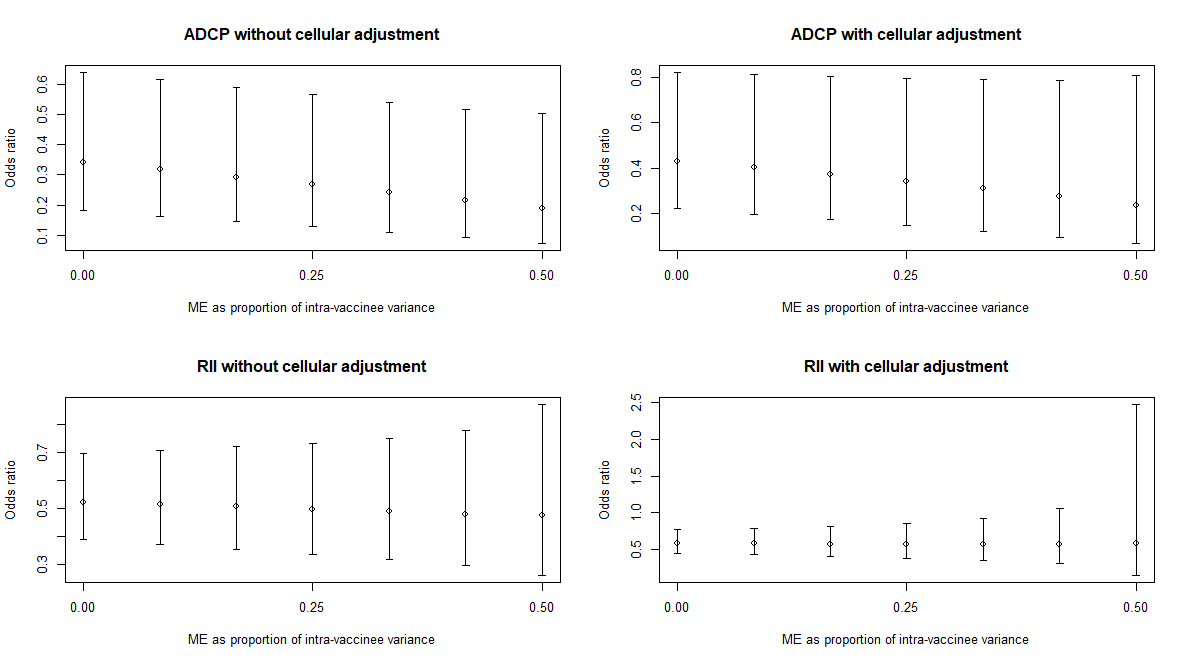
\includegraphics[width=5.9in]{Figure2.png}
\caption{Application results. Each panel shows the results of the DR estimator for the main effect of ADCP or R\RNum{2} in their respective models in the form of odds ratios and confidence intervals. The x-axis reflects increasing user-specified variance of measurement error for the exposures as a proportion of the observed intra-vaccinee exposure variance.}
\label{fig:two}
\end{figure}

The analysis results are plotted in Figure~\ref{fig:two}. For each exposure and each model, the left-most interval in each panel corresponds to the DR estimator under no measurement error. These results are similar to that found in \citet{neidich2019} when using outcome regression to adjust for confounding, but slightly further from the null value in general. The results for the ADCP variable seem robust to measurement error, with significant results even under high measurement error variance. The results for RII are somewhat robust to measurement error, with the confidence intervals in the cellular adjustment model including the null value under moderate measurement error and becoming quite wide under high measurement error. The data for HVTN 505 is publicly available at \href{https://atlas.scharp.org/cpas/project/HVTN\%20Public\%20Data/HVTN\%20505/begin.view?}{https://atlas.scharp.org/} and the R code for the simulations and application are provided at \href{https://github.com/bblette1/causalCSME}{https://github.com/bblette1/causalCSME}.

\section{Discussion}

In this paper, estimators were proposed which adjust for both confounding and measurement error and which are consistent without any supplemental data and without specifying strong distributional or extrapolation assumptions. The proposed methods are semi-parametric in that while parametric assumptions for the errors were made, the true exposures were treated as nuisance parameters and no assumptions were made about their distribution. While the proposed methods were shown to have favorable theoretical and empirical properties, they are not without limitation. In particular, the methods only work without supplemental data if the covariance of measurement error is known or has been previously estimated. As demonstrated in Section 5, if the covariance is unknown then sensitivity analysis can be straightforward and highly informative if the covariance matrix is small or restricted such that it has few parameters. In addition, in order to perform inference without making strong assumptions on $\bm{A}$, modeling assumptions on $\bm{A}^{*}$ and $Y$ that may be implausible in some settings were necessary. However, additive measurement error models are realistic for many variables and the GLM outcome framework is an extremely common statistical analysis procedure used in many fields.

There are many possible extensions of the methods described in this paper. Methods that accommodate different measurement error model forms and more flexible outcome model specifications would be useful. Generalizations of the conditional score approach to broader semiparametric frameworks such as that described in \citet{tsiatis2004} could be adapted to the causal setting to address this and weaken some of the parametric assumptions made in this paper. A version of this idea is proposed by \citet{liu2017}, but the authors take an outcome regression approach to adjusting for confounding, which is often insufficient for causal inference.

Another logical extension would be a g-estimation based estimator that builds off the CSME method to estimate parameters of a structural nested model where at least one exposure is measured with error. In addition, while this paper expands on the conditional score estimation procedure described in \citet{stefanski1987}, the corrected score estimation procedure described in \citet{nakamura1990} also belongs to the score equation family of functional methods, can also correct for measurement error without supplemental data, and has advantages and disadvantages compared to the conditional score approach in various settings. A causal extension of the corrected-score approach would be valuable for many applications. Finally, this paper focuses on point-exposure data, but conditional-score based approaches addressing measurement error and data sparsity for longitudinal and survival data have been described and could be extended to define new causal inference methods in those settings.

This paper adds to a growing literature on addressing measurement error in causal inference problems. No measurement error of any variables is a key assumption in drawing causal inference, but is often left implicit in analyses despite being critical to the identification of causal estimands. Indeed, exposure measurement error is common in observational studies where investigators lack control of the exposure variables - the same conditions in which investigators worry about confounding bias. Methodological contributions at this intersection are needed to facilitate simultaneous adjustment for these prevalent issues.

%  The \backmatter command formats the subsequent headings so that they
%  are in the journal style.  Please keep this command in your document
%  in this position, right after the final section of the main part of
%  the paper and right before the Acknowledgements, Supplementary Materials,
%  and References sections.




\backmatter

%  This section is optional.  Here is where you will want to cite
%  grants, people who helped with the paper, etc.  But keep it short!

\section*{Acknowledgements}

The authors thank Kayla Kilpatrick, Shaina Mitchell, Sam Rosin, Bonnie Shook-Sa, and Jaffer Zaidi for helpful comments and suggestions, as well as the investigators, staff, and participants of the HVTN 505 trial. This work was supported by NIH grant. \vspace*{-8pt}

%  If your paper refers to supplementary web material, then you MUST
%  include this section!!  See Instructions for Authors at the journal
%  website http://www.biometrics.tibs.org

\section*{Supplementary Materials}

The Web Appendix is available with this paper at the Biometrics website on Wiley Online Library.\vspace*{-8pt}

%  Here, we create the bibliographic entries manually, following the
%  journal style.  If you use this method or use natbib, PLEASE PAY
%  CAREFUL ATTENTION TO THE BIBLIOGRAPHIC STYLE IN A RECENT ISSUE OF
%  THE JOURNAL AND FOLLOW IT!  Failure to follow stylistic conventions
%  just lengthens the time spend copyediting your paper and hence its
%  position in the publication queue should it be accepted.

%  We greatly prefer that you incorporate the references for your
%  article into the body of the article as we have done here
%  (you can use natbib or not as you choose) than use BiBTeX,
%  so that your article is self-contained in one file.
%  If you do use BiBTeX, please use the .bst file that comes with
%  the distribution.

\bibliographystyle{biom}
\bibliography{refs}

%\begin{thebibliography}{}

%\end{thebibliography}

\label{lastpage}

\end{document}

